\documentclass{fast_latex}

\usepackage{inputenc}
\usepackage{lastpage}
\usepackage{setspace}
\usepackage{graphicx}
\usepackage[pdfborder={0 0 0}]{hyperref}		% turn on when latex is used (not miktec)
\usepackage{url} % LEO: urls \url{}
\usepackage{verbatim} % code and comment
\usepackage{longtable}
\usepackage{xspace}   % whitespace after a macro if no punctuation after the macro
\usepackage{multirow}
\usepackage{colortbl}
\usepackage{longtable}
\usepackage{array}
\usepackage{amssymb}

% This helps to get hyphenation in typewriter font (\texttt)
\usepackage[htt]{hyphenat}

\parindent0pt

\newcommand\deliverableNumber{D5.1.1}
\newcommand\deliverableTitle{User Manual of the FAST Catalogue}
\newcommand\deliverableTitleShort{Catalogue User Manual}
\newcommand\workpackageNumber{5}
\newcommand\workpackageTitle{Semantic catalogue of screen-flow resources and back-end Web Services}
\newcommand\authorOne{Ciprian Palaghita, Cyntelix}
\newcommand\authorTwo{Ismael Rivera, NUIG}
\newcommand\authorThree{Author 3}
\newcommand\authorFour{Author 4}
\newtheorem{example}{\emph{Example}}

\begin{document}
% explicit hyphenations
\hyphenation{RDF-Re-po-si-to-ry}
\hyphenation{name-space}

%\fontfamily{tahoma}\selectfont
\def\note#1{\marginpar{\footnotesize#1}} % use this to show the notes in the document
%\def\note#1{} % use this to hide the notes


\newenvironment{definition}{}{}

%%%%%%%%%%%%%%%%%%%%%%%%%%%%%%%%%%%%%%%%%%%%%%%%%%%%%%%%%%%%%%%%%%%%%%%%%%%%%%%%
% TITLE PAGES 
%%%%%%%%%%%%%%%%%%%%%%%%%%%%%%%%%%%%%%%%%%%%%%%%%%%%%%%%%%%%%%%%%%%%%%%%%%%%%%%%
\thispagestyle{empty}

\pagenumbering{roman}

\begin{flushright}
	
\includegraphics[width=3cm]{images/FP7_logo}
\end{flushright}

\vspace{1cm}

%\begin{minipage}[p]{15cm}
	\begin{center}
		
\includegraphics{images/FAST_logo}\\
		\vspace{1cm}
		{\LARGE{\sffamily \emph{FAST AND ADVANCED STORYBOARD TOOLS}}}\\
		\vspace{0.5cm}
		{\LARGE \sffamily \emph{FP7-ICT-2007-1-216048}}\\
		\vspace{0.5cm}
		{\LARGE \sffamily \emph{http://fast.morfeo-project.eu}}\\
		\vspace{4cm}
		{\LARGE \sffamily \textbf{Deliverable \deliverableNumber}}\\
		\vspace{0.5cm}
		{\LARGE \sffamily \textbf{\deliverableTitle}}\\
		\vspace{2cm}
		{\large \sffamily \authorOne}\\
		\vspace{0.2cm}
		{\large \sffamily \authorTwo}\\
		\vspace{0.5cm}
		\vfill
		{\large \sffamily Date: 19/02/2010}\\
		\vspace{1cm}
		{\sffamily FAST is partially funded by the E.C. (grant code: FP7-ICT-2007-1-216048).}
		
	\end{center}
%\end{minipage}


\clearpage
%%%%%%%%%%%%%%
% NEXT PAGES %
%%%%%%%%%%%%%%
\pagestyle{scrheadings}

\lohead{
\includegraphics[width=4cm]{images/FAST_logo_transparent}}
%\cohead{\small\textcolor{fast@lightgrey}{\deliverableTitle}}
\rohead{\small{\today}}
%\lofoot{\small\textcolor{fast@lightgrey}{Task Force Ontologies}}
\cofoot{\small{FAST 216048 --- \deliverableTitleShort}}
\rofoot{\small{\thepage}}

\newpage

\clearpage

\section*{Version History}

\begin{small}
\begin{tabular}{|l|l|l|p{6.6cm}|}
\hline
\rowcolor{fast@lightgrey}\textcolor{white}{\textbf{Rev. No.}} &
                         \textcolor{white}{\textbf{Date}} &
                         \textcolor{white}{\textbf{Author (Partner)}} &
                         \textcolor{white}{\textbf{Change description}}\\ \hline
1.0 & 19/02/2010 & Ciprian Palaghita (Cyntelix) & First version of the deliverable \\
 & & Ismael Rivera (NUIG) & \\ \hline
\end{tabular}
\end{small}

\color{black}

\vfill
%{\bf Explanations of abbreviations on front page}\\
%\\
%%Nature \\
%R: Report \\
%P: Prototype \\
%R/P: Report and Prototype \\
%O: Other \\
% \\
%Dissemination level \\
%PU: Public \\
%PP: Restricted to other FP6 participants \\
%RE: Restricted to specified group \\
%CO: Confidential, only for NEPOMUK partners \\

\newpage

%%%%%%%%%%%%%%%%%%%%%
% Executive Summary %
%%%%%%%%%%%%%%%%%%%%%

\clearpage

\section*{Executive Summary}
\doublespacing

The present deliverable is intented to be the developer's manual of the prototype of the semantic catalogue. That said, whoever developing a component which will interact with the catalogue will find in this document a description of its architecture, the functionality provided together with the API (Application Programming Interface), data interchange formats, code errors and exceptions as well as several examples of usage.

\newpage

%%%%%%%%%%%%%%%%%%%%%
% Document Summary %
%%%%%%%%%%%%%%%%%%%%%

\clearpage

\section*{Document Summary}
% double spacing from here on:
\singlespacing

\begin{small}
\begin{tabular}
	%{| >{\columncolor{fast@lightgrey}}p{3.25cm}|p{6cm}|p{2cm}|p{2cm}|}
	{| >{\columncolor{fast@lightgrey}}p{3.25cm}|p{6cm}|p{2cm}|p{2cm}|}
	\hline
	\textcolor{white}{\textbf{Code}} & {FP7-ICT-2007-1-216048} & {\textbf{Acronym}} & {FAST}\\ \hline
	\textcolor{white}{\textbf{Full title}} & \multicolumn{3}{l|}{Fast and Advanced Storyboard Tools}\\ \hline
	\textcolor{white}{\textbf{URL}} & \multicolumn{3}{l|}{\url{http://fast.morfeo-project.eu}}\\ \hline
	\textcolor{white}{\textbf{Project officer}} & \multicolumn{3}{l|}{Annalisa Bogliolo}\\ \hline
\end{tabular}
\end{small}

\vspace{0.5cm}

\begin{small}
\begin{tabular}
	{| >{\columncolor{fast@lightgrey}}p{3.25cm}|p{1.25cm}|p{1cm}|p{1cm}|p{6.32cm}|}
	\hline
	\textcolor{white}{\textbf{Deliverable}} & {\textbf{Number}} & {\deliverableNumber} & {\textbf{Name}} & {\deliverableTitle}\\ \hline
	\textcolor{white}{\textbf{Work package}} & {\textbf{Number}} & {\workpackageNumber} & {\textbf{Name}} & {\workpackageTitle}\\ \hline
\end{tabular}
\end{small}

\vspace{0.5cm}

\begin{small}
\begin{tabular}
	{| >{\columncolor{fast@lightgrey}}p{3.25cm}|p{1.4cm}|p{3.2cm}|p{1.6cm}|p{3.37cm}|}
	\hline
	\textcolor{white}{\textbf{Delivery data}} & {\textbf{Due date}} & {27/02/2010} & {\textbf{Submitted}} & {27/02/2010}\\ \hline
	\textcolor{white}{\textbf{Status}} & \multicolumn{2}{l|}{} & \multicolumn{2}{l|}{final}\\ \hline
	\textcolor{white}{\textbf{Dissemination Level}} & \multicolumn{4}{l|}{Public $\boxtimes$ / Consortium $\square$}\\ \hline
	\textcolor{white}{\textbf{Short description of contents}} & \multicolumn{4}{p{10.85cm}|}{This deliverable is the technical documentation for the prototype developed as part of the WP5. It describes the catalogue's architecture, data interchange formats, APIs and examples of how to interact with it.}\\ \hline
	\textcolor{white}{\textbf{Authors}} & \multicolumn{4}{l|}{\authorOne}\\
	{} & \multicolumn{4}{l|}{\authorTwo}\\ 
%	{} & \multicolumn{4}{l|}{\authorOne}\\ 
%	{} & \multicolumn{4}{l|}{\authorOne}\\
  \hline
	\textcolor{white}{\textbf{Deliverable Owner}} & \multicolumn{2}{l|}{Cyntelix} & \textbf{email} & {cpalaghita@cyntelix.com} \\ \cline{4-5}
	\textcolor{white}{\textbf{(Partner)}} & \multicolumn{2}{l|}{} & \textbf{phone} & {+353 858494258} \\ \hline
	\textcolor{white}{\textbf{Keywords}} & \multicolumn{4}{p{10.85cm}|}{FAST, semantic catalogue, gadget catalogue, RDF store}\\ \hline
\end{tabular}
\end{small}

\newpage

%%%%%%%%%%%%%%%%%%%%%
% TABLE OF CONTENTS %
%%%%%%%%%%%%%%%%%%%%%
\doublespacing
\setcounter{tocdepth}{2}
\tableofcontents
\cleardoublepage
\pagenumbering{arabic}

\clearpage
\listoftables

\clearpage
\listoffigures

%%%%%%%%%%%%%%%%%%%%%%%%%
% BEGINNING OF SECTIONS %
%%%%%%%%%%%%%%%%%%%%%%%%%
\rofoot{\small{Page \thepage\ of \pageref{LastPage}}} 

\clearpage
\section{Introduction} % (fold)
\label{sec:introduction}
This section starts establishing the goal and scope of the present document, shows how it is structured and details the relation to others documents and work packages.

\subsection{Goal and Scope} % (fold)
\label{sub:goal_and_scope}

This is an introductory manual for developers who want to adopt and use the FAST semantic catalogue. It explains the main functionalities implemented so far, an overview of its architecture and a detailed \emph{Application Programming Interface} or API of the complete set of the operations offered through a REST service.

% subsection goal_and_scope (end)

\subsection{Structure of the document} % (fold)
\label{sub:structure_of_the_document}

The deliverable presents both the external and internal architecture in Section~\ref{sec:architecture_overview}, then in Section~\ref{sec:restful_catalogue_api} it is detailed the Catalogue API, query formats, interchange formats, error codes and so on.

% subsection goal_and_scope (end)

\subsection{Changes from previous version} % (fold)
\label{sub:changes_from_previous_version}

This is the first version of this deliverable since in M12 the deliverable 5.1 was not scheduled. Nevertheless, last year an extra document was written as an appendix to the FAST Catalogue in order to detail and clarify technical decisions and to have a technical reference manual, which the content was taken from as the initial draft the present deliverable. Hence, the deliverable D5.2.1 will evolve to become the D5.1.1, so it will be no longer needed by itself.

There are several new sections and major changes which need to be mentioned:

\begin{itemize}
	\item Section~\ref{sec:installation_guide}. Installation Guide describes a set of steps to be followed in order to install and execute the FAST Catalogue. Also some configuration instructions are specified.
	\item Section~\ref{sub:linked_data}. Content Negotiation states how the FAST Catalogue has adopted several of the content negotiation principles.
	\item Section~\ref{sec:restful_catalogue_api}. RESTful Catalogue API has been intensively extended and modified in order to  reflect all the new functionality and how every request or response is constructed. Some of the most important features added in this iteration are:
	\begin{itemize}
		\item support for forms, operators and back-end services (see Section ...),
		\item convenience operations for recommendation and checking satisfaction and reachability for forms, operators and back-end services (see Section ...),
		\item and, last but not least, support for Screen planning (see Section~\ref{sub:planning}).
	\end{itemize}
	\item Several appendixes have been added with the JSON structure of every building block the Catalogue can deal with.
	\item Appendix A. Last year an evaluation to choose the best technology for the Catalogue was done. It was not included in any formal deliverable, so this year it has been documented as an appendix.
\end{itemize}

% subsection changes_from_previous_version (end)

% section introduction (end)

\clearpage
\section{Installation Guide} % (fold)
\label{sec:installation_guide}

This section  provides instructions on how to manually install and configure the FAST Catalogue. The first part of this guide presents some requirements to be considered before the installation, then it gives broad general instructions, and the last part contains a more detailed installation notes for specific configurations.

\subsection{System Requirements} % (fold)
\label{sub:system_requirements}

In addition to the software itself, a standard FAST Catalogue installation has the following requirements:
\begin{itemize}
  \item Java\footnote{http://java.sun.com/} (version 6 or later) is required to run the software.
  \item A Java Servlet Container that supports Java Servlet API 2.4 and Java Server Pages (JSP) 2.0, or newer. We recommend using a recent, stable version of Apache Tomcat\footnote{http://tomcat.apache.org/}. At the time of writing, this is either version 5.5.x or 6.x.
\end{itemize}

In addition, there are various optional dependencies which are required if you want to use certain advanced features (see Section~\ref{sub:installation_instructions}).

% subsection system_requirements (end)

\subsection{Obtaining the FAST catalogue} % (fold)
\label{sub:obtaining_the_fast_catalogue}

It is recommended to have a Subversion client installed before you download the code (although you can theoretically download files without Subversion, this would mean tediously downloading each individual file manually). The recommended software is the official Subversion client, available from the Subversion project page\footnote{http://subversion.tigris.org/}. Note that this client uses a command-line interface, which the instructions below use. Alternatively, you can get subversioning software with a graphical user interface such as TortoiseSVN.

To download from the latest release (recommended), enter the following command from the command-line in the directory you wish to download to:
\begin{verbatim}
svn checkout https://svn.forge.morfeo-project.org/fast-fp7project/trunk/catalogue_service
\end{verbatim}

% subsection obtaining_the_fast_catalogue (end)

\subsection{Installation Instructions} % (fold)
\label{sub:installation_instructions}

Once you have got the source code, first step should be addressed is its compilation. You may manually compile the source yourself, however the FAST Catalogue comes along with a script to facilitate this task. This script has been made using a Java build tool called Ant \footnote{http://ant.apache.org/}. Hence, we recommended to get and install such a tool in order to follow the instructions below.

Now you can compile, package and run the application via:
\begin{verbatim}
ant clean
ant prepare
ant compile
\end{verbatim}

Or using a task which gather the previous three tasks and creates WAR file ready to distribute or deploy:
\begin{verbatim}
ant dist
\end{verbatim}

After executing with no errors this task, a WAR file should have been created in the /dist directory. A WAR file, which stands for  Web Application Archive, is just a JAR file used to distribute a collection of JavaServer Pages, servlets, Java classes, XML files, tag libraries and static Web pages (HTML and related files) that together constitute a Web application, in this case, the FAST Catalogue.

Note that it is also possible to get the compiled WAR file directly from the SVN server. This file can be located at \url{https://svn.forge.morfeo-project.org/fast-fp7project/distribution/catalogue}.

Then, last step is to deply the WAR file into the servlet container. If the server chosen was Apache Tomcat, the procedure for deploying a Web application is:
\begin{enumerate}
	\item Stop Tomcat.
	\item Delete existing deployment. If you have previously deployed "foo.war" in TOMCAT\_HOME/webapps, then it has been unpacked into webapps/foo/... You must delete this directory and all its contents. On Unix, this can be done with
rm -r \$TOMCAT\_HOME/webapps/foo
	\item Copy WAR file to TOMCAT\_HOME/webapps/.
	\item Start Tomcat.
\end{enumerate}

Now you have successfully built the FAST catalogue, however we highly recommend you to read Section~\ref{sub:configuration} and tune your FAST Catalogue instance.

% subsection installation_instructions (end)

\subsection{Configuration} % (fold)
\label{sub:configuration}

The following section covers the configuration options you may have to set up before start using the Catalogue. The FAST Catalogue relies on a Sesame repository for the persistent storage. Sesame repositories can be local or remote. Remote does not mean, it has to be installed in a different machine, but in a servlet container such as Apache Tomcat. The advantage of remote repositories is the possibility of accessing it via a SPARQL endpoint. These configuration aspect can be found in the file \emph{repository.properties} in the root directory where the Catalogue has been deployed.

Independently the type of repository, the parameter \emph{serverURL} needs to take the value of the URL where the FAST Catalogue instance has been deployed. If you are testing the application in your machine, it may be something like \url{http://catalogueURL/FASTCatalogue}.

Local repositories just need the parameter \emph{storageDir} pointing at a local directory, which has write permission in order to allow Sesame to create files in that directory or to delete any file in the directory. For instance:

\begin{verbatim}
storageDir=D:\\FAST\\catalogue\\repository
\end{verbatim}

Nevertheless, setting up a remote repository requires a few more steps. First the OpenRDF Sesame Server needs to be installed. The installation guide of this server is detailed in the Chapter 5 and 6 of the User Guide for Sesame 2.2 \cite{sesame2.2}. Once the Sesame server is deployed, and a repository has been created, the parameters sesameServer and repositoryID will take the values of the Sesame server URL and the repository identifier. For instance:

\begin{verbatim}
sesameServer=http://localhost:8880/openrdf-sesame
repositoryID=c2
\end{verbatim}

% subsection installation_instructions (end)

\subsection{Hello World!} % (fold)
\label{sub:hello_world}

It is recommended to check if the FAST Catalogue has been successfully installed. To do that, a simple HTTP request, using a Web browser, can be sent to the URL the Catalogue is deployed, and specifying a type of resource such as Screen. The URL would be similar to \url{http://catalogueURL/FASTCatalogue/screens}. Depending on the variant chosen, the response may be different. For JSON, the response should be \verb|[]|, but in HTML the message \verb|No screens found.| should be shown.

% subsection hello_world (end)

% section installation_guide (end)


\clearpage
\section{Architecture Overview} % (fold)
\label{sec:architecture_overview}

This section presents a technical overview of the internal catalogue's architecture and which external components will interact with it. Basically three layers can be distinguished: Presentation, Business Logic and Persistence layer (see Figure~\ref{fig:catalogue_architecture}). 

\begin{figure}[htb]
\label{fig:catalogue_architecture}
\begin{center}
	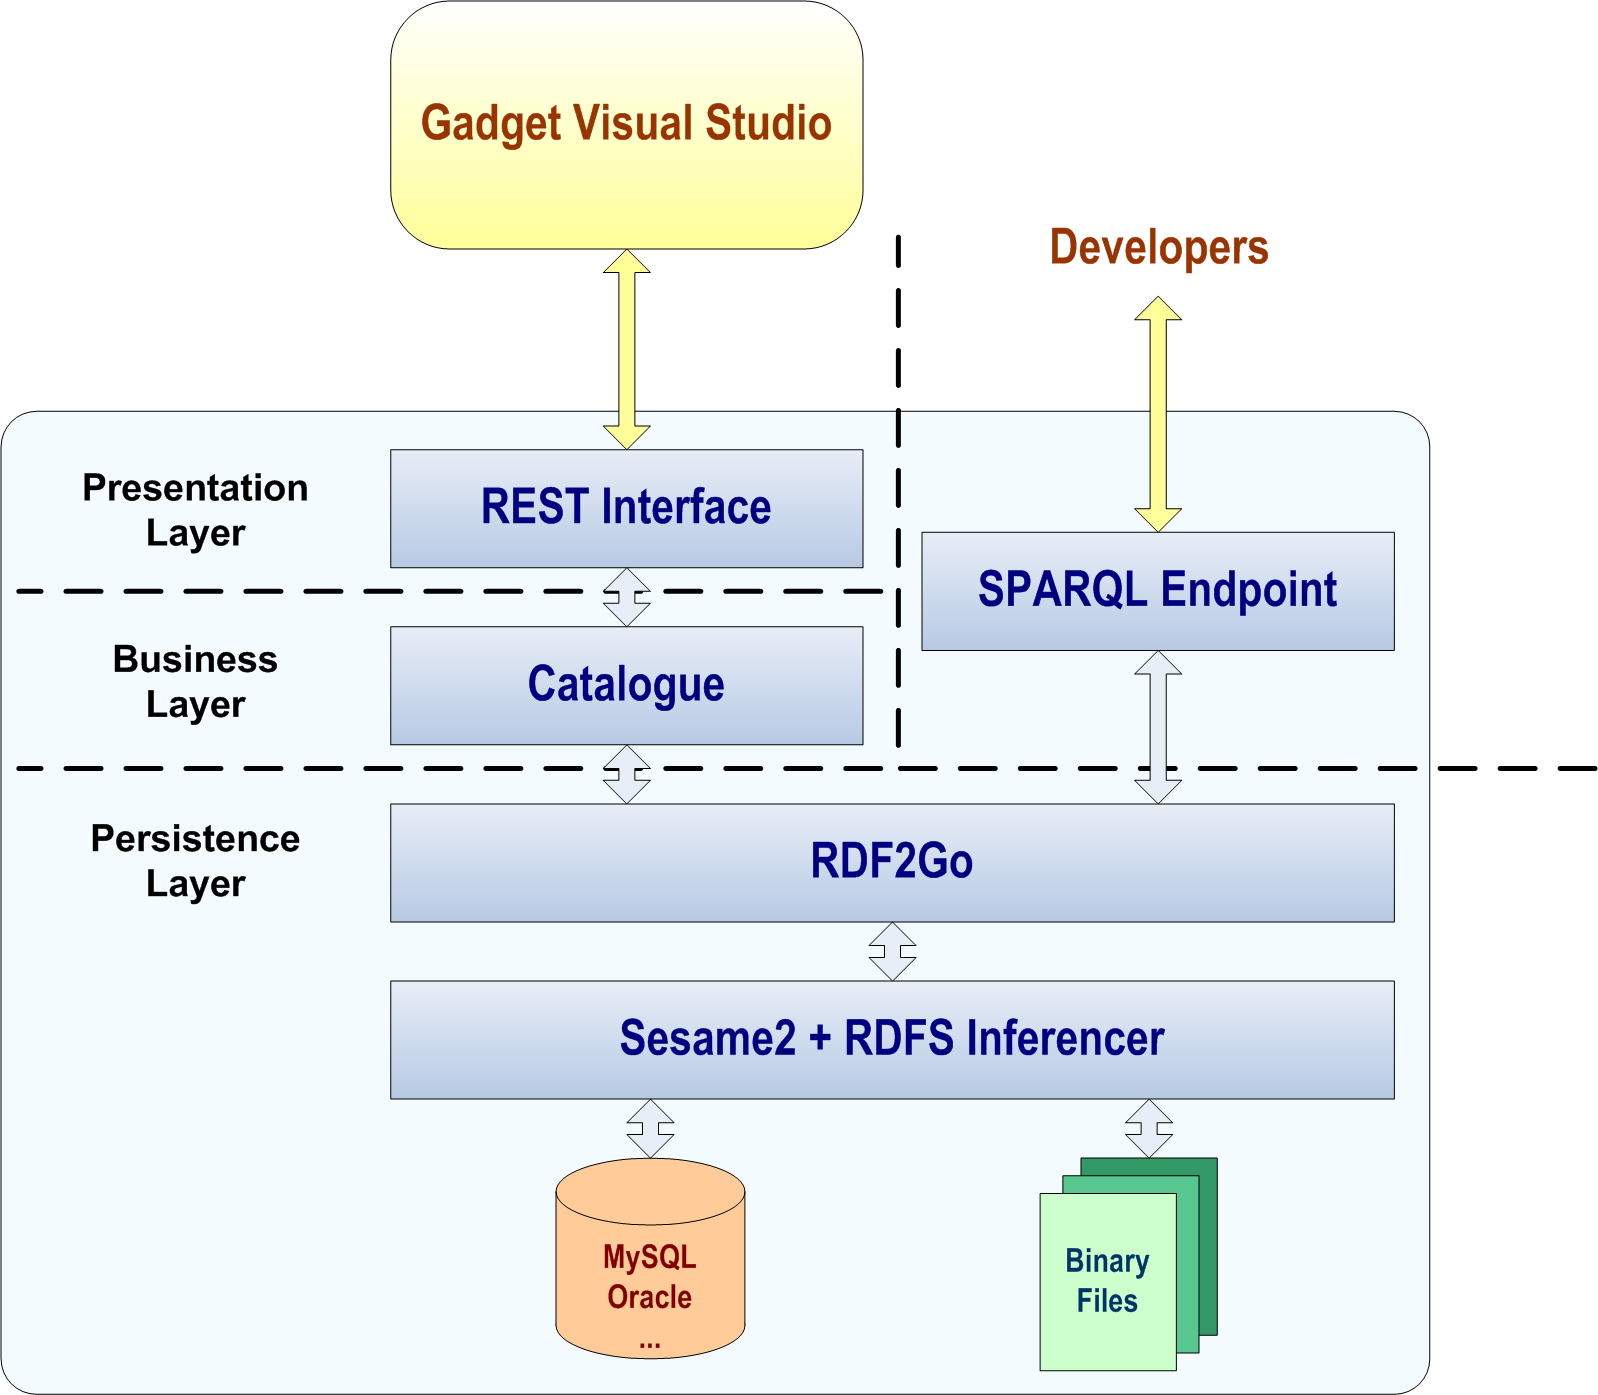
\includegraphics[width=12cm]{images/catalogue_architecture}
	\caption{Catalogue's Architecture}
\end{center}
\end{figure}

The Presentation layer will be the public interface of the catalogue. The main purpose of this layer is to provide its functionality to other components within the Gadget Visual Studio. The service is offered in a REST (REpresentational State Transfer) style, making it easy to consume than other complex APIs. REST is an architectural style, not a toolkit or a standard. Even though, it makes use of standards like HTTP, URI, Resource Representations (XML, HTML, JSON, JPEG, etc.) or MIME types (text/xml, text/html, application/json, image/jpeg, etc.). Another characteristic of the REST style is its stateless assumption. The catalogue adopts this strategy; therefore every request needs a complete set of information in order to prepare the response.

As part of the Presentation layer, a SPARQL endpoint is offered using the SPARQL protocol service as defined in the SPROT \cite{sprot} specification. The SPARQL endpoint is mostly offered to enable other developers to query directly the catalogue knowledge base using SPARQL queries. This feature is supported by the Sesame RESTful HTTP interface for SPARQL Protocol for RDF.

The Business Logic layer contains all the FAST domain-specific processing. It provides functions to interact with all the elements of the domain model specified in \cite{moeller2009fast_ontology}. It processes the input from the Presentation layer, creating specific objects modelling the business logic, and vice versa. In addition it interacts with the Persistence layer in order to persist the model.

The Persistence layer provides an API which allows the Business layer to work with a standard set of objects that read and save their state to the triple store. For this reason, on top of this layer it is used RDF2Go, an abstraction over triple (and quad) stores. The RDF2Go API allows interacting with the semantic representation of the model (triples) in a generic manner, and also brings the flexibility of choosing different triple stores to persist them. The selected implementation for the triple stored is Sesame 2. Moreover, this framework is completely extensible and configurable regarding to storage mechanisms, inferencers, RDF file formats, query result formats and query languages. For the actual catalogue prototype, the storage mechanism used is the native file storage system of Sesame, the inferencer used is a subset of the RDFS entailment rules \cite{rdfsrules} following a forward-chaining policy. 

% section architecture_overview (end)


\clearpage
\section{RESTful Catalogue API} % (fold)
\label{sec:restful_catalogue_api}

This section provides a high-level overview of the Catalogue API. It describes the calls or operations supported, specific parameters and responses for each operation, supported interchange formats and some examples to facilitate the understanding of the API.


\subsection{JSON Interchange Format} % (fold)
\label{sec:json_interchange_format}

The format supported, and in which they must be constructed, by every HTTP request is JSON\footnote{http://www.json.org/}. JSON is a lightweight data interchange format whose simplicity has resulted in widespread use among web developers, easy to read and write and able to using any programming language because its structures map directly to data structures used in most programming languages.

Every HTTP request should be encoded using the MIME type \texttt{application/json} and the charset \texttt{UTF-8}.

The following is an example of a Find \& Check request:

\singlespacing
\begin{verbatim}
{
  "canvas": [
    { "uri": "http://catalogueURL/catalogue/screens/238" },
    { "uri": "http://catalogueURL/catalogue/screens/323" }
  ],
  "elements": [
    { "uri": "http://catalogueURL/catalogue/screens/636" }
  ],
  "domainContext": {
    "tags": [
      {
        "label": { "en-GB": "Amazon" },
        "means": "http://dbpedia.org/page/Amazon.com"
      }
    ],
    "user": "irivera",
  },
  "criterion": "reachability"
}
\end{verbatim}
\doublespacing

\subsubsection{Internationalisation I18n} % (fold)

In order to offers an adaptable solution to various languages and regions without major engineering changes, internationalisation is considered from an early stage in the catalogue development. Underlying representation technologies used to develop the catalogue (RDF/XML and JSON) allow to implement this feature. This feature is implemented by the addition of a language tag to every 'string' desired. The specification of this language tag is composed by the language code and the country code, following the ISO 639\footnote{http://ftp.ics.uci.edu/pub/ietf/http/related/iso639.txt} for languages and the ISO 3166\footnote{http://userpage.chemie.fu-berlin.de/diverse/doc/ISO\_3166.html} for countries. The following example illustrates how to use it properly in both formats.

\singlespacing
\begin{verbatim}
{
  "label": {
    "en-GB": "Product Search",
    "es-ES": "B�squeda de productos",
    "de-DE": "Produktsuche"
  },
  "description": {
    "en-GB": "On this screen, the user can enter a search term.",
    "es-ES": "En esta ventana, el usuario puede introducir el criterio de b�squeda",
    "de-DE": "Auf diesem Screen kann der Benutzer einen Suchbegriff eingeben."
  }
}
\end{verbatim}
\doublespacing

\singlespacing
\begin{verbatim}
<rdf:RDF
    xmlns:rdf="http://www.w3.org/1999/02/22-rdf-syntax-ns#"
    xmlns:foaf="http://xmlns.com/foaf/0.1/"
    xmlns:dc="http://purl.org/dc/terms/"
    xmlns:fgo="http://purl.oclc.org/fast/ontology/gadget#"
    xmlns:xsd="http://www.w3.org/2001/XMLSchema#"
    xmlns:rdfs="http://www.w3.org/2000/01/rdf-schema#"
    xmlns:ctag="http://commontag.org/ns#">
  <rdf:Description rdf:about="http://demo.fast.morfeo-project.org/FASTCatalogue/screens/1">
    <rdf:type rdf:resource="http://purl.oclc.org/fast/ontology/gadget#Screen"/>
    <rdfs:label xml:lang="en-gb">Product Search</rdfs:label>
    <rdfs:label xml:lang="en-es">B�squeda de productos</rdfs:label>
    <rdfs:label xml:lang="en-de">Produktsuche</rdfs:label>
    <dc:description xml:lang="en-gb">On this screen, the user can enter a search
    term.</dc:description>
    <dc:description xml:lang="en-gb">En esta ventana, el usuario puede introducir
    el criterio de b�squeda.</dc:description>
    <dc:description xml:lang="en-gb">Auf diesem Screen kann der Benutzer einen
    Suchbegriff eingeben.</dc:description>
  </rdf:Description>
</rdf:RDF>
\end{verbatim}
\doublespacing

Internationalisation is being used by the attributes \emph{label} and \emph{description} of any building block, \emph{label} of the pre/postconditions and \emph{label} of the tags.

% subsection json_interchange_format (end)

\subsection{Linked Data} % (fold)
\label{sub:linked_data}

Apart from serving as the back-end system for the Gadget Visual Storyboard (GVS), the catalogue publishes all FAST building blocks as linked data, following the principles as originally defined in \cite{bernersLee2006linkedData}, in order to make them available to arbitrary third party applications. Each building block is identified by an HTTP URI and hosted through the catalogue so that it can be dereferenced through the same URI. For each building block, data is available in representations in different standard formats such as JSON (for communication with the GVS), RDF/XML, Turtle, or even HTML+RDFa as a human-readable version. 
Following the principles and best practices proposed in \cite{berrueta2008} and \cite{sauermann2008cool_uris}, these representations are served based on the request issued by the requesting agent, using a technique called \emph{content negotiation}.
As required by the forth rule of linked data, individual building blocks link to other data on the Web, thereby preventing so-called isolated ``data islands''.

In order to understand how content negotiation is implemented in the catalogue, a few concepts need to be understood. The URI of a particular building block must be understood as the identifier of the building block as such, as opposed to a particular representation (JSON, HTML, etc.) of it. In fact, each such representation has its own URI, under which it can be retrieved. Using the terminology established in \cite{w3c2004webArchitecture}, the building block is a \emph{non-information resource}, whereas each representation is an \emph{information resource}. In the process of content negotiation, the requesting agent will first request the URI of the building block as such (e.g., \texttt{http://catalogue.com/screens/235}), as well as the required representation format (e.g., JSON). The catalogue will then inspect the request and redirect the requester to the appropriate representation (e.g., \texttt{http://catalogue.com/screens/235.json}), as illustrated in Fig.~\ref{fig:content_negotiation}.
On the Web, different representations for the same resource are called \emph{variants}, and content negotiation is the mechanism used to determine which of the representations of most appropriate for a given request.

\begin{figure}[htb]
\label{fig:content_negotiation}
\begin{center}
	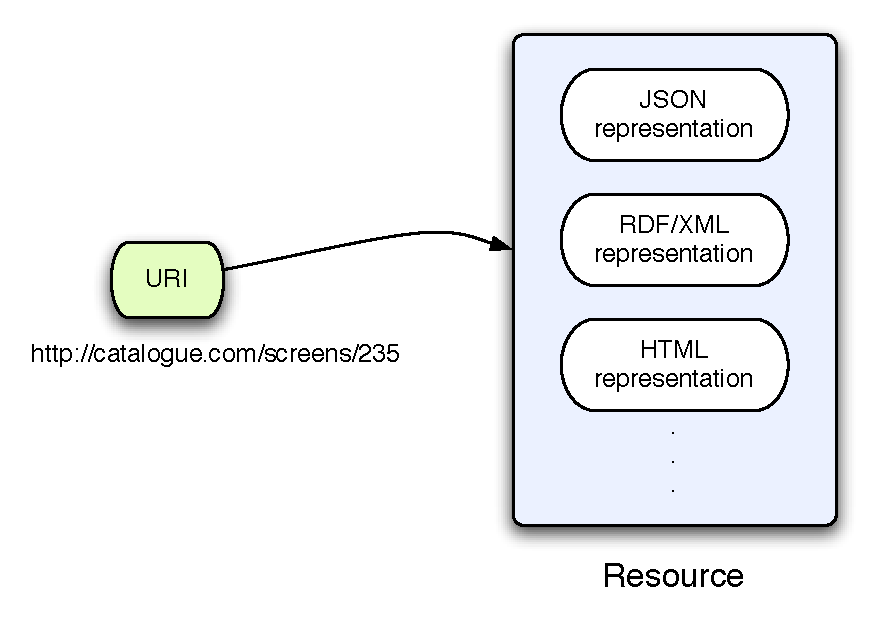
\includegraphics[width=12cm]{images/content_negotiation}
	\caption{Content Negotiation}
\end{center}
\end{figure}

In summary, the basic idea of content negotiation, as stated in the \cite{http1.1}, is to serve the best variant for a resource, taking into account what variants are available, what variants the server may prefer to serve, what the client can accept, and with which preferences. In HTTP, this is done by the client which may send, in its request, accept headers (\texttt{Accept}, \texttt{Accept-Language} and \texttt{Accept-Encoding}), to communicate its capabilities and preferences in format, language and encoding, respectively.

In fact, what the catalogue really does is ``format negotiation'' since the alternate representations are just based on the selection of the media type, through the accept header, but does not consider different languages or encoding types. The formats supported are JSON, RDF/XML, Turtle and HTML+RDFa. Even though the accept header is desired, the different representations can also be retrieved directly by dereferencing their own URI. The convention used in the catalogue for deriving a representation URI from a building block URI is to simply attach a matching suffix, such as \texttt{.rdf}, \texttt{.json} or \texttt{.html}.

Lastly, content negotiation needs to identify which player is going to take the lead on it. There are two kinds of content negotiation which are possible in HTTP: server-driven and agent-driven negotiation. The approach followed by the catalogue is agent-driven negotiation, hence selecting a specific representation for a resource is responsibility of the user agent. If none is specified, by default, the server will choose the JSON representation.

% subsection content_negotiation (end)

\subsection{API Calls} % (fold)
\label{sub:api_calls}

This section contains detailed descriptions of the interface provided by the catalogue via REST services, detailing request parameters, response elements, any special errors and examples of requests and responses. The URL format is also specified for each operation, where 'catalogueURL' has to be replaced for the real URL the service is installed (e.g. http://demo.fast.morfeo-project.org/catalogue).

\subsubsection{CRUD operations} % (fold)

Any building block within the Catalogue is a resource in terms of REST philosophy, hence it can be created, retrieved, modified or deleted, using a certaing URL and a specific HTTP method for every operation. Two concepts have to be defined: \emph{collection}, as a set of resources which access URI is http://catalogueURL/<type>/ where catalogueURL is the specific URL where the Catalogue server is installed and <type> is the plural of the name of the building block (e.g. screens, services), and \emph{member} of the collection, in other words, the building block itself, which access URI is http://catalogueURL/<type>/<id> where the <id> has to be replaced by the identifier of a specific building block. The details of the operations and which HTTP verb has to be used can be found in the Table~\ref{tab:crud_operations}.

\begin{table}[htb]
\caption{CRUD operations}
\label{tab:crud_operations}
\begin{center}
\begin{tabular}{|p{2.5cm}|p{2.5cm}|p{3.5cm}|p{5cm}|}
\hline
\rowcolor{fast@lightgrey}\textcolor{white}{Resource} &
                         \textcolor{white}{HTTP method} &
                         \textcolor{white}{HTTP body} &
                         \textcolor{white}{Description}\\ \hline
Collection URI & GET & N/A & \textbf{List} the members of the collection.\\ \hline
Collection URI & PUT & N/A & Not used.\\ \hline
Collection URI & POST & JSON representation of the building block & \textbf{Create} a new entry in the collection where the URI is assigned automatically by the collection. The URI created is returned by this operation.\\ \hline
Collection URI & DELETE & N/A & Not used.\\ \hline
Member URI & GET & N/A & \textbf{Retrieve} the addressed member of the collection.\\ \hline
Member URI & PUT & JSON representation of the building block & \textbf{Update} the addressed member of the collection or create it with a defined URI.\\ \hline
Member URI & POST & N/A & Not used. \\ \hline
Member URI & DELETE & N/A & \textbf{Delete} the addressed member of the collection.\\ \hline
\end{tabular}
\end{center}
\end{table}

The JSON structure for create any building bock can be found in the appendixes. All of them are composed of a common structure which can be found in Section Appendix B, and some specific information depending on the type. Screen-flows are defined in Appendix C, screens in Appendix D and forms, operators and back-end services share the same structure detailed in Appendix E. However, a few examples of request and responses are shown in order to clarify how the request are constructed and sent, and how the responses look like.

To create a new screen, a POST request is sent to the catalogue server, concretely to \texttt{http://cata\-logueURL/screens}, including the JSON representation of the screen in the body of the request:

\singlespacing
\begin{verbatim}
{
  "code": "http://demo.fast.morfeo-project.org/code/amazonList.js",
  "creationDate": "2010-01-26T17:01:13+0000",
  "creator": "irivera",
  "description": {"en-gb": "Please fill the description..."},
  "homepage": "http://fast.morfeo-project.eu/",
  "icon": "http://demo.fast.morfeo-project.org/images/amazonList.png",
  "id": "28",
  "label": {"en-gb": "Amazon Product List"},
  "name": "ProductList",
  "postconditions": [
    [
      {
        "id": "item",
        "label": { "en-gb": "An item" },
        "pattern": "?I 
                    http://www.w3.org/1999/02/22-rdf-syntax-ns#type
                    http://aws.amazon.com/AWSECommerceService#Item",
        "positive": "true"
      }
    ]
  ],
  "preconditions": [
    [
      {
        "id": "filter",
        "label": { "en-gb": "A search criteria" },
        "pattern": "?F
                    http://www.w3.org/1999/02/22-rdf-syntax-ns#type
                    http://aws.amazon.com/AWSECommerceService#SearchCriteria",
        "positive": "true"
      }
    ]
  ],
  "rights": "http://creativecommons.org/",
  "screenshot": "http://demo.fast.morfeo-project.org/images/amazonProductList.png",
  "tags": [{"label": {"en-gb": "amazon"}}],
  "version": "0.1"
}
\end{verbatim}
\doublespacing

The URI of the screen is created using the id specified in the JSON request. So, the response for this operation is:

\singlespacing
\begin{verbatim}
{
  "code": "http://demo.fast.morfeo-project.org/code/amazonList.js",
  "creationDate": "2010-01-26T17:01:13+0000",
  "creator": "irivera",
  "description": {"en-gb": "Please fill the description..."},
  "homepage": "http://fast.morfeo-project.eu/",
  "icon": "http://demo.fast.morfeo-project.org/images/amazonList.png",
  "id": "28",
  "label": {"en-gb": "Prueba1"},
  "name": "ProductList",
  "postconditions": [
    [
      {
        "id": "item",
        "label": { "en-gb": "An item" },
        "pattern": "?I
                    http://www.w3.org/1999/02/22-rdf-syntax-ns#type
                    http://aws.amazon.com/AWSECommerceService#Item",
        "positive": "true"
      }
    ]
  ],
  "preconditions": [
    [
      {
        "id": "filter",
        "label": { "en-gb": "A search criteria" },
        "pattern": "?F
                    http://www.w3.org/1999/02/22-rdf-syntax-ns#type
                    http://aws.amazon.com/AWSECommerceService#SearchCriteria",
        "positive": "true"
      }
    ]
  ],
  "rights": "http://creativecommons.org/",
  "screenshot": "http://demo.fast.morfeo-project.org/images/amazonProductList.png",
  "tags": [{"label": {"en-gb": "amazon"}}],
  "type": "screen",
  "uri": "http://catalogueURL/catalogue/screens/28",
  "version": "0.1"
}
\end{verbatim}
\doublespacing

To obtain all the screens stored in the catalogue a HTTP GET request is sent to the Collection URI and the response may be something like this:

\singlespacing
\begin{verbatim}
[
  {
    "code": "http://demo.fast.morfeo-project.org/code/amazonList.js",
    "creationDate": "2010-01-26T17:01:13+0000",
    "creator": "irivera",
    "description": {"en-gb": "Please fill the description..."},
    "homepage": "http://fast.morfeo-project.eu/",
    "icon": "http://demo.fast.morfeo-project.org/images/amazonList.png",
    "id": "28",
    "label": {"en-gb": "Prueba1"},
    "name": "ProductList",
    "postconditions": [
      [
        {
          "id": "item",
          "label": { "en-gb": "An item" },
          "pattern": "?I
                      http://www.w3.org/1999/02/22-rdf-syntax-ns#type
                      http://aws.amazon.com/AWSECommerceService#Item",
          "positive": "true"
        }
      ]
    ],
    "preconditions": [
      [
        {
          "id": "filter",
          "label": { "en-gb": "A search criteria" },
          "pattern": "?F
                      http://www.w3.org/1999/02/22-rdf-syntax-ns#type
                      http://aws.amazon.com/AWSECommerceService#SearchCriteria",
          "positive": "true"
        }
      ]
    ],
    "rights": "http://creativecommons.org/",
    "screenshot": "http://demo.fast.morfeo-project.org/images/amazonProductList.png",
    "tags": [{"label": {"en-gb": "amazon"}}],
    "type": "screen",
    "uri": "http://catalogueURL/catalogue/screens/28",
    "version": "0.1"
  },
  {
    "creationDate": "2009-02-07T09:59:52+0000",
    "creator": "fabio",
    ...,
	  "uri": "http://catalogueURL/catalogue/screens/14",
    "version": "1.0"
  },
  {
    "creationDate": "2009-02-07T09:59:52+0000",
    "creator": "javier",
    ...,
	  "uri": "http://catalogueURL/catalogue/screens/564",
    "version": "1.0"
  }
]
\end{verbatim}
\doublespacing

\subsubsection{Screen Find} % (fold)
\label{ssub:screen_find}

The find operation searches inside the catalogue for any screen which could be somehow related to the gadget the user is creating. It provides a recommended set of screens depending on the domain context, the canvas, and so on.

The specific URL to access this operation is http://catalogueURL/screens/find using HTTP POST method. From now on, the method 'find' only considers the domain context and the pre/postconditions of the screens. It will try to satisfy all the unsatisfied preconditions of a given list of screens also known as canvas. The results will be all the screens stored in the catalogue which fulfil some of these preconditions, and are tagged with the tags specified in the domain context. The request parameters are shown in Table~\ref{tab:screen_find_request} and the response parameters are shown in Table~\ref{tab:screen_find_response}.

\begin{table}[htb]
\caption{Screen Find Request Parameters}
\label{tab:screen_find_request}
\begin{center}
\begin{tabular}{|p{2.5cm}|p{9cm}|p{2cm}|}
\hline
\rowcolor{fast@lightgrey}\textcolor{white}{Name} &
                         \textcolor{white}{Description} &
                         \textcolor{white}{Type}\\ \hline
canvas & The canvas is composed by a list of screens. Only the URI is needed. & Optional \\ \hline
domainContext & The domain context contains a list of tags and a user. & Optional \\ \hline
elements & It is a list of resources, previously stored in the catalogue. For example, the list of screens recommended last execution. Only accepts screens. & Optional \\ \hline
\end{tabular}
\end{center}
\end{table}

\begin{table}[htb]
\caption{Screen Find Response Parameters}
\label{tab:screen_find_response}
\begin{center}
\begin{tabular}{|p{2.5cm}|p{9cm}|p{2cm}|}
\hline
\rowcolor{fast@lightgrey}\textcolor{white}{Name} &
                         \textcolor{white}{Description} &
                         \textcolor{white}{Type}\\ \hline
N/A & A list of recommended screens URIs is returned. & Required \\ \hline
\end{tabular}
\end{center}
\end{table}

Following is shown an example of usage of this operation considering a canvas with the screen \texttt{http://catalogueURL/catalogue/screens/654}.

\singlespacing
\begin{verbatim}
{
  canvas: [
    { uri: "http://catalogueURL/catalogue/screens/654" }
  ],
  domainContext: {
    tags: [],
	  user: null
  },
  elements: []
}
\end{verbatim}
\doublespacing

After the execution of the recommendation algorithm, the response given by the catalogue is:

\singlespacing
\begin{verbatim}
[
  "http://catalogueURL/catalogue/screens/371",
  "http://catalogueURL/catalogue/screens/24",
  "http://catalogueURL/catalogue/screens/253",
  "http://catalogueURL/catalogue/screens/12"
]
\end{verbatim}
\doublespacing


\subsubsection{Screen Check} % (fold)
\label{ssub:screen_check}

This operation verifies the state of certain list of screens depending on a specific criterion. The only criterion accepted in this stage of the prototype is 'reachability'. A screen will be reachable if it all its preconditions are satisfied by postconditions of the screens the canvas contain. The specific URL to access this operation is http://catalogueURL/screens/check using HTTP POST method. 

\begin{table}[htb]
\caption{Screen Check Request Parameters}
\label{tab:screen_check_request}
\begin{center}
\begin{tabular}{|p{2.5cm}|p{9cm}|p{2cm}|}
\hline
\rowcolor{fast@lightgrey}\textcolor{white}{Name} &
                         \textcolor{white}{Description} &
                         \textcolor{white}{Type}\\ \hline
canvas & The canvas is composed by a list of screens. Only the URI is needed. & Optional\\ \hline
domainContext & The domain context contains a list of tags and a user. & Optional\\ \hline
elements & It is a list of resources, previously stored in the catalogue. For example, the list of screens recommended last execution. Only accepts screens. & Optional\\ \hline
criterion & The criterion specifies what it has to be check. The only possible supported now is 'reachability' in order to check if the preconditions of a screen are satisfied. & Required\\ \hline
\end{tabular}
\end{center}
\end{table}

\begin{table}[htb]
\caption{Screen Check Response Parameters}
\label{tab:screen_check_response}
\begin{center}
\begin{tabular}{|p{2.5cm}|p{9cm}|p{2cm}|}
\hline
\rowcolor{fast@lightgrey}\textcolor{white}{Name} &
                         \textcolor{white}{Description} &
                         \textcolor{white}{Type}\\ \hline
canvas & The canvas indicating which screens satisfy the critetion. More aditional information may be included, for example, a satisfaction attribute for every precondition for reachability. & Optional\\ \hline
domainContext & The domain context contains a list of tags and a user. & Optional\\ \hline
elements & The elements indicating which satisfy the critetion. More aditional information may be included as in the Canvas. & Optional\\ \hline
\end{tabular}
\end{center}
\end{table}

The scenario for the following example is composed by a screen in the canvas which precondition is a foaf:Person which foaf:workplaceHomepage is \url{http://www.deri.ie/}, and a screen in the elements list which precondition is a foaf:Person. The state to check in this case is the reachability and satisfaction of the screens and preconditions.

\singlespacing
\begin{verbatim}
{
  "canvas": [
    { "uri": "http://catalogueURL/catalogue/screens/238" }
  ],
  "elements": [
    { "uri": "http://catalogueURL/catalogue/screens/636" }
  ],
  "domainContext": {
    "tags": [
      {
        "label": { "en-GB": "Amazon" },
        "means": "http://dbpedia.org/page/Amazon.com"
      }
    ],
    "user": "irivera",
  },
  criterion: "reachability"
}
\end{verbatim}
\doublespacing

The response shows that there are not reachable screens at the moment, and preconditions are not satisfied.

\singlespacing
\begin{verbatim}
{
  "canvas": [{
    "preconditions": [{
      "label": {"en-gb": "A person working in DERI"},
      "pattern": "?person rdf:type foaf:Person . 
                  ?person foaf:workplaceHomepage http://www.deri.ie/",
      "positive": true,
      "satisfied": false
    }],
    "reachability": false,
    "uri": "http://catalogueURL/catalogue/screens/238"
  }],
  "elements": [{
    "preconditions": [{
      "label": {"en-gb": "A person"},
      "pattern": "?person rdf:type foaf:Person",
      "satisfied": false
    }],
    "reachability": false,
    "uri": "http://catalogueURL/catalogue/screens/636"
  }]
}
\end{verbatim}
\doublespacing


\subsubsection{Screen Find \& Check} % (fold)
\label{ssub:screen_findcheck}

For convenience and to minimise the number of request, the Find operation may be combined with the Check operation. This operation will look for new screens based on the given information, and will perform the Check to both the screens in the canvas and the screens in the \emph{elements} attribute.

The format of the request is the same as the one used in the Check operation:

\singlespacing
\begin{verbatim}
{
  "canvas": [
    { "uri": "http://catalogueURL/catalogue/screens/238" }
  ],
  "elements": [
    { "uri": "http://catalogueURL/catalogue/screens/636" }
  ],
  "domainContext": {
    "tags": [
      {
        "label": { "en-GB": "Amazon" },
        "means": "http://dbpedia.org/page/Amazon.com"
      }
    ],
    "user": "irivera",
  },
  criterion: "reachability"
}
\end{verbatim}
\doublespacing

The response for the above request is:

\singlespacing
\begin{verbatim}
{
  "canvas": [{
    "preconditions": [{
      "label": {"en-gb": "A person working in DERI"},
      "pattern": "?person rdf:type foaf:Person . 
                  ?person foaf:workplaceHomepage http://www.deri.ie/",
      "positive": true,
      "satisfied": false
    }],
    "reachability": false,
    "uri": "http://catalogueURL/catalogue/screens/238"
  }],
  "elements": [
    {
      "preconditions": [{
        "label": {"en-gb": "A person"},
        "pattern": "?person rdf:type foaf:Person",
        "satisfied": false
      }],
      "reachability": false,
      "uri": "http://catalogueURL/catalogue/screens/636"
    },
    {
      "preconditions": [],
      "reachability": true,
      "uri": "http://catalogueURL/catalogue/screens/132"
    }
  ]
}
\end{verbatim}
\doublespacing


\subsubsection{GetMetadata} % (fold)

Although the information about a resource can be obtained by its specific retrieval operation supported by the CRUD interface, sometimes is needed to retrieve information which would imply a request per resource, hence this operation allow to get the metadata of a list of resources in only one request. This prototype supports this operation for screen-flows and screens. The specific URL to access this operation is http://catalogueURL/getmetadata using HTTP POST method. Table~\ref{tab:getmetadata_request} shows the parameters needed for the invocation and Table~\ref{tab:getmetadata_response} details the different parameters may contain a response.

\begin{table}[htb]
\caption{GetMetadata Request Parameters}
\label{tab:getmetadata_request}
\begin{center}
\begin{tabular}{|p{2.5cm}|p{9cm}|p{2cm}|}
\hline
\rowcolor{fast@lightgrey}\textcolor{white}{Name} &
                         \textcolor{white}{Description} &
                         \textcolor{white}{Type}\\ \hline
N/A & A list of URIs. & Required\\ \hline
\end{tabular}
\end{center}
\end{table}

\begin{table}[htb]
\caption{GetMetadata Response Parameters}
\label{tab:getmetadata_response}
\begin{center}
\begin{tabular}{|p{2.5cm}|p{9cm}|p{2cm}|}
\hline
\rowcolor{fast@lightgrey}\textcolor{white}{Name} &
                         \textcolor{white}{Description} &
                         \textcolor{white}{Type}\\ \hline
screen-flows & A set of screen-flows with all the metadata associated to them.. & Optional\\ \hline
screens & A set of screens with all the metadata associated to them. & Optional\\ \hline
forms & A set of forms with all the metadata associated to them. & Optional\\ \hline
operators & A set of operators with all the metadata associated to them. & Optional\\ \hline
backendservices & A set of back-end services with all the metadata associated to them. & Optional\\ \hline
\end{tabular}
\end{center}
\end{table}

The following example send two URIs of screens and a URI of a screen-flow to the GetMetadata operation:

\singlespacing
\begin{verbatim}
[
  "http://catalogueURL/catalogue/screens/12",
  "http://catalogueURL/catalogue/screens/48",
  "http://catalogueURL/catalogue/forms/9",
]
\end{verbatim}
\doublespacing

The response obtained are two lists, one containing all the metadata regarding to the screen-flows and another one with the information about the screens:

\singlespacing
\begin{verbatim}
{
  "screenflows": [],
  "screens": [
    {
      "creationDate": "2009-02-07T09:59:52+0000",
      "creator": "irivera",
      ...,
      "uri": "http://catalogueURL/catalogue/screens/12",
      "version": "1.0"
    },
    {
      "creationDate": "2009-02-07T09:59:52+0000",
      "creator": "irivera",
      ...,
      "uri": "http://catalogueURL/catalogue/screens/12",
      "version": "1.0"
    }
  ],
  "forms": [
    {
      "actions": [
        {
          "name": "init",
          "preconditions": [],
          "uses": []
        },
        {
          "name": "showTable",
          "preconditions": [{
            "id": "list",
            "label": {"en-gb": "A product list"},
            "pattern": "?PList
                        http://www.w3.org/1999/02/22-rdf-syntax-ns#type
                        http://aws.amazon.com/AWSECommerceService#ProductList",
            "positive": true
          }],
          "uses": []
        }
      ],
      ...,
      "uri": "http://catalogueURL/FASTCatalogue/forms/9",
      "version": "1.0"
    },
  ],
  "operators": [],
  "backendservices": []
}
\end{verbatim}
\doublespacing

\subsubsection{Screen Component Find \& Check} % (fold)
\label{ssub:screen_component_findcheck}

Similarly to the Screen Find \& Check described in Section~\ref{ssub:screen_findcheck}, this operation search for screen components (forms, operators and back-end services) through the catalogue in order to satisfy a given request, and it will attach information about satisfaction and reachability as well.

A request is formed of the following parameters:

\begin{description}
	\item[preconditions] Preconditions of the screen.
	\item[postconditions] Postcondition of the screen.
	\item[canvas] The canvas is composed by a list of screens. Only the URI is needed.
	\item[forms] It is a list of forms, such as the list of forms recommended last execution.
	\item[operators] It is a list of operators, such as the list of operators recommended last execution.
	\item[backendservices] It is a list of back-end services, such as the list of back-end services recommended last execution.
	\item[search] Boolean indicating if forms/operators/services are required to be looked for. If \emph{false} the operation performed is just a check. If missed, it will act as \emph{true}.
	\item[domainContext] The domain context contains a list of tags and a user.
	\item[pipes] List of pipes for the connection between screen components.
	\item[selectedItem] URI of a screen component from the canvas.
\end{description}

The screen components recommended are based on the given domain context and the pre/postconditions of the any of the resources in the canvas or the conditions of the parameters preconditions and postconditions. Hence, any screen component from the catalogue which has any of these conditions may be suitable for the screen, so it is included in the response, in the list corresponding to the type of screen component.

An example of request is the following:

\singlespacing
\begin{verbatim}
{
  "preconditions": [{
    "id": "Searchcriteria_1",
    "label": {"en-gb": "A search criteria"},
    "pattern": "?F
                http://www.w3.org/1999/02/22-rdf-syntax-ns#type
                http://aws.amazon.com/AWSECommerceService#SearchCriteria",
    "positive": true,
  }],
  "postconditions": [],
  "canvas": [
    { "uri": "http://catalogueURL/catalogue/forms/1" },
    { "uri": "http://catalogueURL/catalogue/services/1" }
  ],
  "forms": [],
  "operators": [],
  "backendservices": [],
  "search": true,
  "domainContext": {
    "tags": [],
    "user": null
  },
  "pipes": [
    {
      "from": {
        "buildingblock": "http://catalogueURL/catalogue/services/1",
        "condition": "list"
      },
      "to": {
        "action": "showTable",
        "buildingblock": "http://catalogueURL/catalogue/forms/1",
        "condition": "list"
      }
    }
  ],
  "selectedItem": "http://catalogueURL/catalogue/forms/1"
}
\end{verbatim}
\doublespacing

And the response according to the above request is:

\singlespacing
\begin{verbatim}
{
  "backendservices": [],
  "canvas": [
    {
      "actions": [{
        "name": "search",
        "preconditions": [{
          "id": "filter",
          "label": {"en-gb": "A search criteria"},
          "pattern": "?F 
                      http://www.w3.org/1999/02/22-rdf-syntax-ns#type
                      http://aws.amazon.com/AWSECommerceService#SearchCriteria",
          "positive": true,
          "satisfied": false
        }],
        "satisfied": false,
        "uses": []
      }],
      "reachability": false,
      "uri": "http://catalogueURL/catalogue/services/1"
    },
    {
      "actions": [
        {
          "name": "init",
          "preconditions": [],
          "satisfied": true,
          "uses": []
        },
        {
          "name": "showTable",
          "preconditions": [{
            "id": "list",
            "label": {"en-gb": "A product list"},
            "pattern": "?PList
                        http://www.w3.org/1999/02/22-rdf-syntax-ns#type
                        http://aws.amazon.com/AWSECommerceService#ProductList",
            "positive": true,
            "satisfied": false
          }],
          "satisfied": false,
          "uses": []
        }
      ],
      "reachability": true,
      "uri": "http://catalogueURL/catalogue/forms/1"
    }
  ],
  "connections": [
    {
      "from": {
        "buildingblock": null,
        "condition": "Searchcriteria_1"
      },
      "to": {
        "action": "search",
        "buildingblock": "http://catalogueURL/catalogue/services/1",
        "condition": "filter"
      }
    },
  ],
  "forms": [],
  "operators": [],
  "pipes": [
    {
      "from": {
        "buildingblock": "http://catalogueURL/catalogue/services/1",
        "condition": "list"
      },
      "satisfied": true,
      "to": {
        "action": "showTable",
        "buildingblock": "http://catalogueURL/catalogue/forms/1",
        "condition": "list"
      }
    }
  ],
  "postconditions": []
}
\end{verbatim}
\doublespacing

For a screen component to be reachable, its preconditions need to be connected by a pipe to any other screen component which is already reachable, or to any of the screen preconditions. Moreover, the pipe needs to be satisfied, in other words, conditions in both edges are compatible.

The response includes an attribute called "connections". This attribute will be retrieved when "selectedItem" is given, and it will contain a list of potential pipes to connect to that item.

% subsubsection screen_component_findcheck (end)

% subsection api_calls (end)

\subsection{Planning}
\label{sub:planning}

While creating a screen-flow, the user need to find proper screens which will satisfy her necessity. Once the user has selected one or several screens to be included in her screen-flow, she needs to find screens which satisfy the preconditions of these screens, in order to create an executable screen-flow. The operation Find, detailed in Section~\ref{ssub:screen_find}, helps the user to find these screens, however the response is just a set of screens which somehow may help to accomplish her goal, but not in a single and straight-forward step.

This functionality offers to the user the possibility to receive a whole set of screens, or plan, which will make a given screen, or goal, reachable. These plans take into account the screen which are already in the canvas, in order to minimise the number of screens.

The specific URL to access this operation is \url{http://catalogueURL/planner}, and to execute the operation a POST request needs to be done. The request body is composed of:

\begin{description}
	\item[goal] Required. URI of the goal screen.
	\item[canvas] Required. List of screens URIs.
	\item[page] Optional. Number of the page to be retrieved.
	\item[per\_page] Optional. Number of plans to be included per page in the response.
\end{description}

Let's see the following example:

Request
\singlespacing
\begin{verbatim}
{
  "goal": "http://catalogueURL/catalogue/screens/35",
  "canvas": [
    { "uri": "http://catalogueURL/catalogue/screens/56" },
    { "uri": "http://catalogueURL/catalogue/screens/85" }
  ],
  "page": 1,
  "per_page": 10 
}
\end{verbatim}
\doublespacing

Response
\singlespacing
\begin{verbatim}
[
  [
    "http://catalogueURL/catalogue/screens/13",
    "http://catalogueURL/catalogue/screens/23"
  ],
  [
    "http://catalogueURL/catalogue/screens/79",
    "http://catalogueURL/catalogue/screens/37",
    "http://catalogueURL/catalogue/screens/14"
  ],
  [
    "http://catalogueURL/catalogue/screens/16",
    "http://catalogueURL/catalogue/screens/44",
    "http://catalogueURL/catalogue/screens/32"
  ]
]
\end{verbatim}
\doublespacing

The response is ranked based on adding the minimum number of new screens into the canvas, and giving preference to the screens the user has previously selected (canvas).

In the above example, let's assume the first plan is using the two screens from the canvas to accomplish the goal, and the second plan is able to make the goal reachable by itself. That said, a screen-flow with the goal and the second plan could be executable, and it would be composed of just four screens, however, taking the first plan, the resulting screen-flow will be composed of five screens. It could make sense to place the second plan in first position, but the plan with just two screens reuse the screens from the canvas which has been added by the user.

% subsection planning (end)

\subsection{API Error Codes} % (fold)
There are two types of error codes, client and server.
\begin{itemize}
	\item Client error codes are generally caused by the client and might be an invalid domain or an invalid request parameter. These errors are accompanied by a 4xx HTTP response code. For example: ResourceNotFound.
	\item Server error codes are generally caused by a server-side issue and should be reported. These errors are accompanied by a 5xx HTTP response code. For example: ServerUnavailable.
\end{itemize}

The following table lists all the error codes.

\begin{table}[htb]
\caption{API Error Codes}
\begin{center}
\begin{tabular}{|p{3.5cm}|p{7cm}|p{3cm}|}
\hline
\rowcolor{fast@lightgrey}\textcolor{white}{Error} &
                         \textcolor{white}{Description} &
                         \textcolor{white}{HTTP Status Code}\\ \hline
ResourceNotFound & The resource <resourceURI> has not been found. & 404 Not Found \\ \hline
AccessFailure & Access to the resource <resourceName> is denied. & 403 Forbidden \\ \hline
InternalError & Request could not be executed due to an internal service error. & 500 Internal Server Error \\ \hline
InvalidAction & The action <actionName> is not valid for this web service.  & 404 Bad Request \\ \hline
InvalidHttpRequest & The HTTP request is invalid. Reason: <reason>. & 400 Bad Request \\ \hline
InvalidLiteral & Illegal literal in the filter expression. & 400 Bad Request \\ \hline
InvalidParameterValue & The specified parameter value is not valid. & 400 Bad Request \\ \hline
InvalidURI & The URI <requestURI> is not valid. & 400 Bad Request \\ \hline
MissingAction & No action was supplied with this request. & 400 Bad Request \\ \hline
MissingParameter & The request must contain the specified missing parameter. & 400 Bad Request \\ \hline
NotYetImplemented & Feature <feature> is not yet available. & 401 Unauthorized \\ \hline
ServiceUnavailable & The service is currently unavailable. Please try again later. &  \\ \hline
UnsupportedHttpVerb & The requested HTTP verb is not supported: <verb>. & 400 Bad Request \\ \hline
URITooLong & The URI exceeded the maximum limit of <maxLength>. & 400 Bad Request \\ \hline
\end{tabular}
\end{center}
\end{table}


\clearpage
\bibliographystyle{apalike}
\bibliography{fast_d5_1_1}


\clearpage
\section*{Appendix A. Semantic Web Technologies Evaluation}
\label{appendix_a}
\addcontentsline{toc}{section}{Appendix A. Semantic Web Technologies Evaluation}

In \cite{urmetzer2010fast_state_of_the_art} were presented different technologies used in the Semantic Web community regarding Web services and catalogues or repositories. These are potential technologies to serve as the basis for the Catalogue implementation. Said that, an evaluation was done in order to choose the most accurate technology with the most advantages for it. Of particular importance in this evaluation is real-time performance, because the GVS (Gadget Visual Storyboard) actually relies on the Catalogue in parts of its user interface.

Basically, two general solutions were considered. One was to build the Catalogue, and the internal components or building block of the gadgets, based on a dedicated SWS platform. The other was to build a light-weight solution from scratch based on RDF and RDFS.

For both solutions, a few ideas about their potential benefits and disadvantages were in mind beforehand. SWS platforms were very tempting to use, because the modelling approach for screens in FAST is quite similar to SWS, in how they define their inputs and outputs. E.g., both FAST and WSMO have pre- and post-conditions, OWL-S has inputs/outputs. Also, SWS platforms come with ready-made implementations for service composition, which could have been used for automatically combining screens to screen-flows. On the downside, it was expected that SWS platforms a bit too slow for some FAST requirements, as the need of real-time discovery. On the other hand, building a light-weight implementation directly on RDFS promised to be faster. Moreover, there is a broader, more mature and probably more active tool support. However, going in this direction would imply to invest a lot more work in modelling and implementation efforts, since all the features that SWS would bring straight away are could not be reused.

To perform the evaluation of the different approaches, an abstract random ontology of 40 concepts was created. About 70\% of those were randomly assigned to be sub-concepts of other concepts. The abstract ontology was instantiated in WSMO, OWLS and RDFS. Then, 3 sample sets of random screens of three different sizes (100, 1000 and 10000) were created, such that each screen has 0..3 random pre- and post-conditions. For each set in each technology, every screen was taken to perform a match with any other screen, and the average response time was measured. Figure~\ref{fig:comparison_chart} shows the results of the evaluation (RDFS in blue, WSMO in yellow and OWL-S in green). Be aware that the scale of the time is logarithmic.

\begin{figure}[htb]
\label{fig:comparison_chart}
\begin{center}
	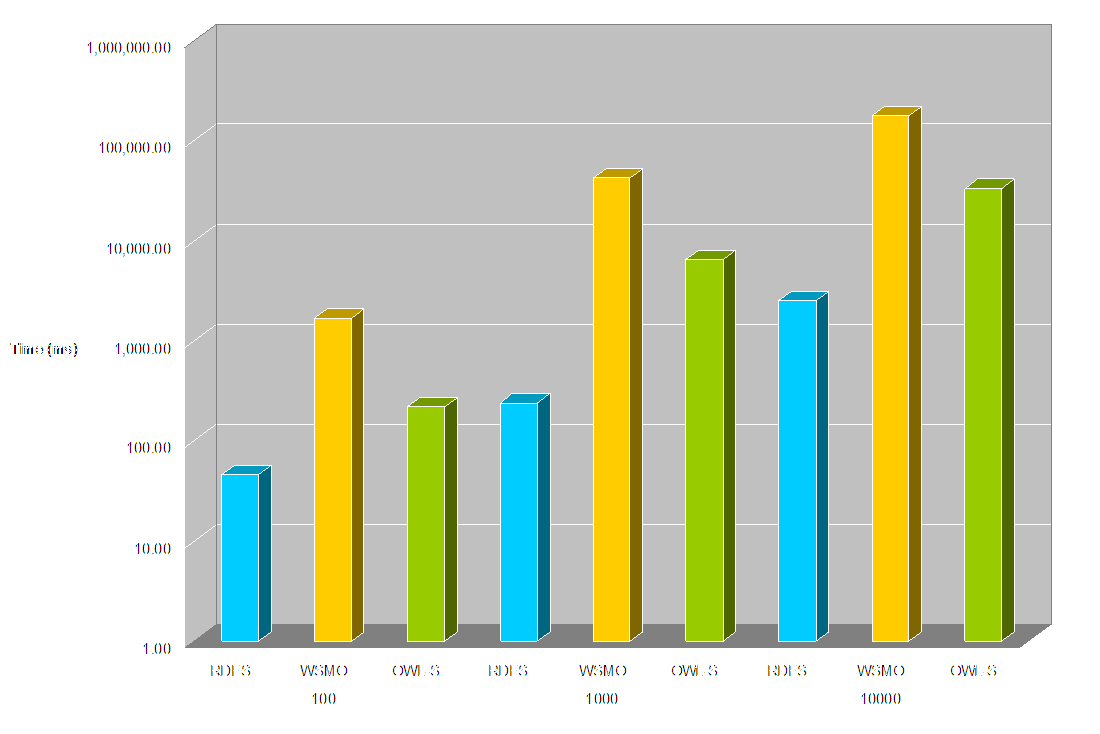
\includegraphics[width=14cm]{images/comparison_chart}
	\caption{Semantic Web Technologies Performance Comparison}
\end{center}
\end{figure}

It can be seen that RDFS performs rather well, even in the 10.000 size set, whereas the other two are pretty far behind. E.g., average response times for WSMO is > 1.5 sec already for the smallest 100 size set. Hence, based on this evaluation the approach to follow for the implementation was RDFS, since WSMO and OWL-S simply could not give the performance required for the real-time discovery.


\clearpage
\section*{Appendix B. Generic Building Block JSON Structure}
\label{appendix_b}
\addcontentsline{toc}{section}{Appendix B. Generic Building Block JSON Structure}

\singlespacing
\begin{verbatim}
{
  "code": "http://url.com/.../code.js",
  "creationDate": "2009-04-20T17:00:00+0100",
  "creator": "username",
  "description": {"en-gb": "This is a description of the building block"},
    "tags":[
      {
        "label":{"en-gb":"Amazon"},
        "means":"http://dbpedia.org/page/Amazon.com"
      },
      {
        "label":{"en-gb":"eBay"},
        "means":"http://dbpedia.org/page/Ebay"
      }
    ],
  "homepage": "http://url.com/.../homepage",
  "icon": "http://url.com/images/.../icon.png",
  "id": "Id of the building block", // i.e. 3545
  "label": {"en-gb": "Label or title of the building block"},
  "name": "User-friendly name of the building block",
  "rights": "http://creativecommons.org/",
  "screenshot": "http://url.com/.../screenshot.jpg",
  "type": "type of the building block", // screenflow, screen, form, operator or resource
  "uri": "http://url.com/screens/525",
  "version": "1.0"
}
\end{verbatim}
\doublespacing


\clearpage
\section*{Appendix C. Screen-flow JSON Structure}
\label{appendix_c}
\addcontentsline{toc}{section}{Appendix C. Screen-flow JSON Structure}

\singlespacing
\begin{verbatim}
{
  <GENERIC BUILDING BLOCK JSON>,
  "contains": [
    "http://url.com/screens/72723",
    "http://url.com/screens/20035",
  ],
}
\end{verbatim}
\doublespacing


\clearpage
\section*{Appendix D. Screen JSON Structure}
\label{appendix_d}
\addcontentsline{toc}{section}{Appendix D. Screen JSON Structure}

\singlespacing
\begin{verbatim}
{
  <GENERIC BUILDING BLOCK JSON>,
  "postconditions": [[{
    "id": <identifier:String>,
    "label": {"en-gb": "Purchase URL"},
    "pattern": "?P
                http://www.w3.org/1999/02/22-rdf-syntax-ns#type
                http://aws.amazon.com/AWSECommerceService#PurchaseURL",
    "positive": true
  }]],
  "preconditions": [[{
    "id": "cart",
    "label": {"en-gb": "A shopping cart"},
    "pattern": "?C
                http://www.w3.org/1999/02/22-rdf-syntax-ns#type
                http://aws.amazon.com/AWSECommerceService#ShoppingCart",
    "positive": true
  }]],
  "code": "URL of the code",
  "definition": {
    "buildingblocks: [
      { // Form
        "id": "form1", // unique for the container screen
        "uri": "http://purl.oclc.org/fast/ontology/gadget#Form670238"
      },
      { // Operators
        "id": "op1",
        "uri": "http://purl.oclc.org/fast/ontology/gadget#Operator213487"
      },
      {  // Backend services
        "id": "bs1",
        "uri": "http://purl.oclc.org/fast/ontology/gadget#Backendservice38399"
      },
      {...}
    ]
    "pipes": [
      {
        "from": {
          "buildingblock": "bs1",
          "condition": "cA"
        },
        "to": {
          "buildingblock": "op1",
          "condition": "cA", // can be the same id, unique for the building block
          "action": "filter"
        }
      },
    "triggers": [
      {
        "from": {
          "buildingblock": "form1",
          "name": "refresh"
        },
        "to": {
          "buildingblock": "bs1",
          "action": "list"
        }
      }
    ]
  }
}
\end{verbatim}
\doublespacing


\clearpage
\section*{Appendix E. Screen Component JSON Structure}
\label{appendix_e}
\addcontentsline{toc}{section}{Appendix E. Screen Component JSON Structure}

\singlespacing
\begin{verbatim}
{
  <GENERIC BUILDING BLOCK JSON>,
  "actions": [{
    "name": "filter",
    "preconditions": [[{
      "id": "item",
      "label": {"en-gb": "Ebay List"},
      "pattern": "?Item
                  http://www.w3.org/1999/02/22-rdf-syntax-ns#type
                  http://aws.amazon.com/AWSECommerceService#Item",
      "positive": true
    }]],
    "uses": [{
      "id":"cart",
      "uri":"http://aws.amazon.com/AWSECommerceService#ShoppingCart"
    }]
  }],
  "libraries": [{
    "language":"JavaScript",
    "source":"http://url.com/libcode.js"
  }],
  "postconditions": [[{
    "id": "filterEbay",
    "label": {"en-gb": "Ebay List"},
    "pattern": "?eFilter
                http://www.w3.org/1999/02/22-rdf-syntax-ns#type
                http://developer.ebay.com/.../FindItemsAdvanced.html#Request",
    "positive": true
  }]],
  "triggers": ["itemAmazon"]
}
\end{verbatim}
\doublespacing

\end{document}
